\chapter{Experimentos y resultados}

Se realizaron 2 tipos de experimentos, de visión y de manipulación. Pruebas de resolución no se llevaron a cabo, ya que el solucionador siempre encuentra una solución, a menos que el cubo se encuentre en un estado inválido.

Se utilizó el scrambler legacy de la World Cube Association, para generar 20 permutaciones del cubo de Rubik. Cada una de estas permutaciones, también llamados ``desarmes'' consiste de 30 rotaciones, y fueron aplicadas manualmente sobre el cubo. La tabla \ref{vision} del apéndice muestra las secuencias de rotaciones utilizadas en cada experimento.

\section{Visión}
Para la visión, se utilizaron los 20 desarmes en su totalidad. Cada ejecución comenzó con el robot recogiendo el cubo desde una mesa.

\begin{figure}[h!]
	\centering
	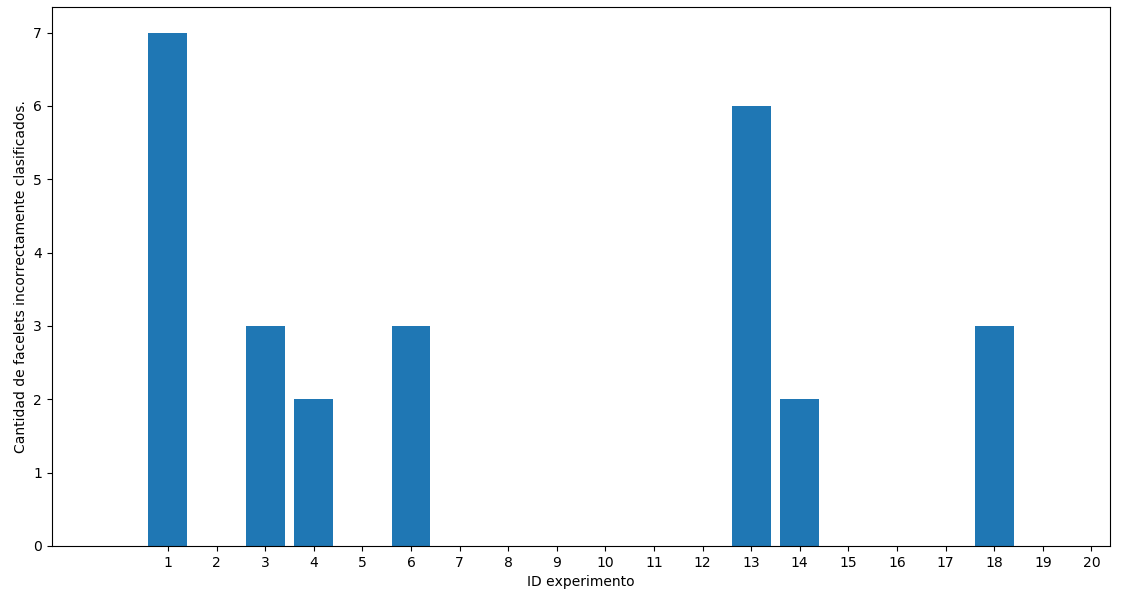
\includegraphics[width=\textwidth]{figures/error_facelet}
	\caption{Facelets mal clasificados por cada prueba realizada.}
	\label{erroresfacelets}
\end{figure}
Del total de pruebas, el 65\% no tuvo errores de clasificación. La cantidad de facelets mal clasificados en promedio fue de 1.3 facelets, con desviación estándar de 2.076. La cantidad de facelets mal clasificados en cada experimento se muestra en la figura\ref{erroresfacelets}. En la tabla\ref{visionerrors} del apéndice, se muestra específicamente cuales fueron los estados del cubo en cada ejecución, y exactamente cúales fueron los faceles indebidamente clasificados.

Respecto a la totalidad de facelets en todos los experimentos, el 97.6\% fue etiquetado correctamente. Lamentablemente, basta con 1 sólo facelet incorrecto para que el solver sea incapaz de encontrar una solución, por lo que en el mejor de los casos el robot hubiese sido capaz de resolver el 65\% de estos desarmes.

\begin{figure}[h!]
	\centering
	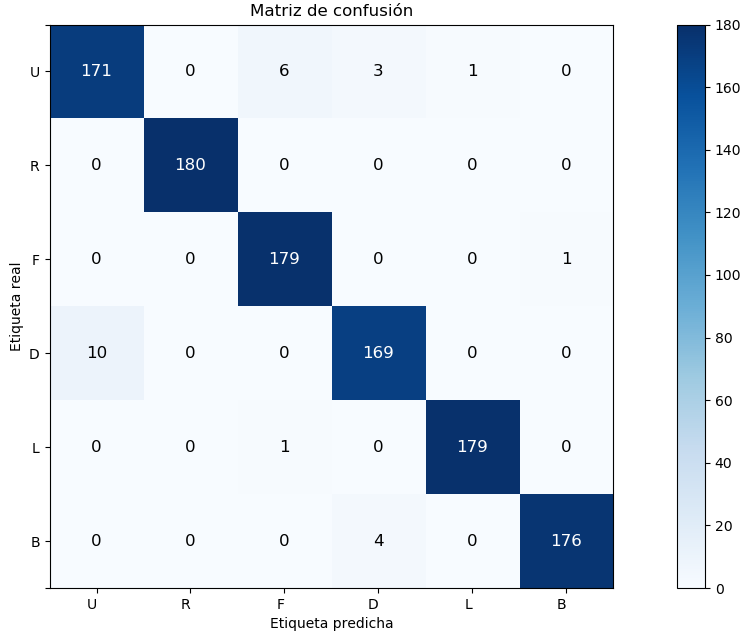
\includegraphics[width=0.7\textwidth]{figures/conf_matrix}
	\caption{Matriz de confusión de predicción de colores, sin normalizar.}
	\label{confusion}
\end{figure}
\begin{figure}[h!]
	\centering
	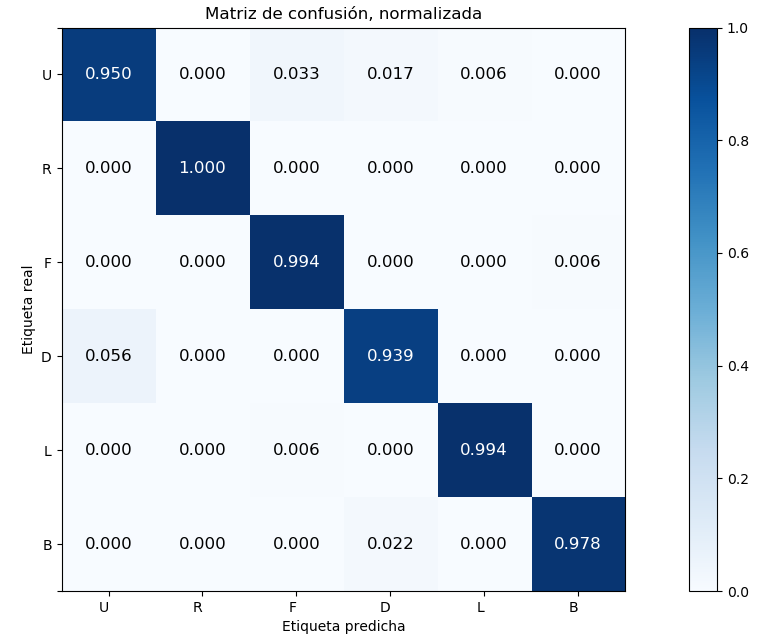
\includegraphics[width=0.7\textwidth]{figures/conf_matrix_norm}
	\caption{Matriz de confusión de predicción de colores, normalizada.}
	\label{confusionnorm}
\end{figure}

Una parte importante de los errores se dieron entre las caras U y D, que en las pruebas realizadas correspondieron a los colores rojo y rosado. Estos colores son muy similares entre sí, aunque esto depende mucho de las condiciones de iluminación del ambiente donde se encuentre el robot. El detalle de los errores por cara se muestra en las figuras\ref{confusion} y \ref{confusionnorm}.



\section{Manipulación}
Para esta clase de pruebas se utilizaron los mismos desarmes que en las pruebas de visión, pero con el desarme $i$ truncado a $i$ rotaciones. De esta manera, se probó una secuencia por cada uno de los largos de secuencias posibles, desde el mínimo (1) hasta el máximo (20). Se midió en cuál giro el robot es incapaz de proseguir. Los resultados se ven en la tabla \ref{resultadogiros}.

\begin{table}[h!]
	\centering
	\begin{tabular}{|r|r|l|}
		\hline
		Largo & Cambios & Resultado \\ \hline \hline
		 1 & 1 & Ejecución completada exitosamente \\ \hline
		 2 & 0 & Ejecución completada exitosamente \\ \hline
		 3 & 1 & Ejecución falla en giro 3 \\ \hline
		 4 & 2 & Ejecución completada exitosamente \\ \hline
		 5 & 2 & Ejecución completada exitosamente \\ \hline
		 6 & 1 & Ejecución completada exitosamente \\ \hline
		 7 & 4 & Ejecución completada exitosamente \\ \hline
		 8 & 2 & Ejecución completada exitosamente \\ \hline
		 9 & 5 & Ejecución falla en giro 6 \\ \hline
		10 & 5 & Ejecución completada exitosamente \\ \hline
		11 & 7 & Ejecución completada exitosamente \\ \hline
		12 & 8 & Ejecución falla en giro 8 \\ \hline
		13 & 10 & Ejecución falla en giro 3 \\ \hline
		14 & 10 & Ejecución falla en giro 4 \\ \hline
		15 & 6 & Ejecución falla en giro 14 \\ \hline
		16 & 8 & Ejecución falla en giro 5 \\ \hline
		17 & 10 & Ejecución falla en giro 10 \\ \hline
		18 & 10 & Ejecución falla en giro 14 \\ \hline
		19 & 11 & Ejecución falla en giro 12 \\ \hline
		20 & 12 & Ejecución falla en giro 8 \\ \hline
	\end{tabular}
	\caption{Resultados experimentos de manipulación. La columna ``largo'' es el largo de la secuencia y la columna ``cambios'' es la cantidad de cambios de mano que debe realizar el robot para ejecutarla.}
	\label{resultadogiros}
\end{table}

Para finalizar, tómense los experimentos previamente presentados con algo de pues dada que la magnitud del espacio de estados del cubo de Rubik es enorme ($\approx 4.5*10^{19}$) ninguna cantidad no astronómica de pruebas será representativa de todas las configuraciones posibles.
